%*******10********20********30********40********50********60********70********80

% For all chapters, use the newdefined chap{} instead of chapter{}
% This will make the text at the top-left of the page be the same as the chapter

\chap{Introduction}\label{chap:introduction}
Children's health has historically always been a sensitive and concerning matter for humankind. We can find the reason for this in our universal instinctive draw towards the protection and care for our offspring, and in how children can be struck by some of the most devastating and life-wrecking diseases. Sometimes, these are the phenotypical expression of genetical marks, scarred onto and into these kids. Despite the origin, the color of the skin or the culture the child bears in his or her lineage, human beings feel the need to raise and safeguard them from all harms, on a physical, emotional and spiritual level. This universal phenomenon is one of the most potent biological calls to action in all human experience.

Thus, pediatrics must care and remember that children's health and well-being must be guarded across political borders, across poverty, across starvation. This thesis, and the paper it's so profoundly bound to set themselves to renew this vow.

\section{Intercountry and international adoptees}\label{sec:internationaladoptees}
International adoptees are children with special needs: a vulnerable pediatric population with a chronic condition that requires access to a wide variety of health care services (as defined by \cite{notonlyinfectious} and \cite{nonsoloinfezioni}); they are recognized as a group of children requiring medical attention (see \cite{caringfor}). Compared to 19\% of the general population, approximately 39\% of adopted children need special healthcare attention (as extensively explained in \cite{nelson}). They are of school age, either part of a sibling group, members of historically oppressed racial or ethnic groups, or have considerable physical, emotional, or developmental need: all potential elements of vulnerability endangering the child's healthy upbringing. This is not a limited problem: annually more than 30.000 kids are adopted across countries, and, in the United States, of all 136.000 national adoptees in 2008, almost 25\% came from foreign countries; U.S. families adopted 22.884 children in 2004, mostly from China (which accounts for 33\% alone), Ethiopia, Russia, and South Korea (see \cite{nelson}), 8.868 more in 2012 and 4.714 in 2017 (see \cite{usreport}). It's estimated that more than 125.000 children have been adopted in the United States alone since 1986 (source can be found in \cite{caringfor}). Further data on annual U.S. international adoptions and their social and financial costs can be found at \cite{usreportsite}. More in-depth medical issues will be discussed in Section \ref{sec:roleofpediatrician}.

Although personal experiences obviously vary, most children placed for international adoption have some history of poverty and social hardship in their home countries, and approximately 65\% are adopted from orphanages or institutional settings (as stated in \cite{caringfor}). As explained in \cite{nelson}, the effects of institutionalization and other early life stress impact all areas of early growth and development. As a result, many children require specialized support and understanding to overcome such impacts and to reach their full potential. 

Moreover, as in \cite{unreport}, internationally adopted children may withstand a number of juridical and social impairments even after adoption. No generalization can be made on this matter though since laws and policies significantly differ among countries. They may be stripped of their name (a.e. in Cape Verde, Argentina and Turkey), have no right to inheritance (a.e. in Republic of Moldova and France), see the termination of the relationship with birth parents and relatives (a.e. in Japan, Albania and Togolese Republic), lose their citizenship and not acquire a new one (a.e. Hungary and New Zealand), or even bear limitations on marriage in their adult life (a.e. in Argentina and France). These boundaries are to be considered associated with the emotional and psychological stress of new surroundings, new affections, new habits, and even new climatic environments.\\
All these elements account for some of the factors that contribute to the hardships an adoptee must endure throughout his life and call for strong action from pediatric physicians and social services employees, as possible support figures which may change these kids' lives forever.

\subsection{Levels and trends in intercountry adoption worldwide}\label{sub:levelsintercountry}
International adoption is increasingly considered a measure of last resort worldwide, applied only if the child's birth family or community are unable or unwilling to care for him anymore (see \cite{nelson}), justifying the downward trend of international adoptions across the globe. 

The United Nations' Population Division estimates that about 40.000 intercountry adoptions took place each year around 2005, accounting for 15\% of the total number of adoptions (see \cite{unreport}). As shown in Table \ref{tab:intadoptcountriesdestination} and \ref{tab:intadoptcountriesorigin}, the involved countries, both for destination and origin, are relatively few.

The United States led destination countries with over 127.000 total adoptions in 2001. Even though it accounts for nearly half of all approvals, only 15\% of American families decide to take care of a child coming from outside the US. France and Spain (both with significant annual adoptions, ranging from 4.000 to 5.000 adoptions per year), instead, embrace 80-90\% of all passages from foreign lands, although they have far less total adoptions per year. Almost all countries adopt primarily from China and Russia. Confirming data are shown in Table \ref{tab:intadoptcountriesorigin}. The median percentage of international adoptions in all examined countries is 64\%: a remarkable value and effort in helping children from developing countries.

The Italian adoption status will be discussed in Section \ref{sub:intadoptioninitaly}.

%International adoption countries of destination
\begin{table}[H]
   \centering
   \begin{tabular}{c l r r l}
      Rank & Receiving country\footnotemark[1] & Number & Percentage & Main country of origin\\
      \hline
      1 & United States of America & 19.056 & 15 & China\\
      2 & France & 3.995 & 90 & Haiti\\
      3 & Spain & 3.951 & 82 & Russia\\
      \textcolor{BrickRed}{\textbf{4}} & \textcolor{BrickRed}{\textbf{Italy}} & \textcolor{BrickRed}{\textbf{2.177}} & \textcolor{BrickRed}{\textbf{68}} & \textcolor{BrickRed}{\textbf{Russia}}\\
      5 & Germany & 1.919 & 34 & Russia\\
      6 & Canada & 1.875 & 46 & China\\
      7 & Sweden & 1.093 & 65 & China\\
      8 & Netherlands & 1.069 & 78 & China\\
      9 & Denmark & 688 & 55 & China\\
      10 & Norway & 664 & 76 & China\\
      11 & Switzerland & 558 & 79 & Colombia\\
      \hline
      \multicolumn{2}{l}{Median} & 370 & 64 &\\
   \end{tabular}
   \caption{Countries of destination with the largest number of intercountry adoption.}
    \source{United Nations Population Division report (see \cite{unreport})}
    \label{tab:intadoptcountriesdestination}
\end{table}

Countries of origin are better balanced throughout the globe, with China leading the chart, followed by Russia, Guatemala, and Ukraine. Guatemala and Ethiopia stand out for the exceptional percentage of international adoptions among all, with 97\% and 93\% respectively. As clearly shown in Table \ref{tab:intadoptcountriesorigin}, the United States is the preferred destination country for most of the listed nations. 

All of the countries listed below struggle with some sort of social hardship: political instability, poverty, inequality, starvation, ethnic or civil wars, complex and violent pasts. Eyes can't be closed and mouths shut, when it so obviously portrayed that children are the ones paying from these adulthood failures. They must run, be saved, separated, deported in order to be granted one single chance, one single hope.

%International adoption countries of origin
\begin{table}[H]
   \centering
   \begin{tabular}{c l r r l}
      Rank & Country of origin\footnotemark[1] & Number & Percentage & Main receiving country\\
      \hline
      1 & China & 8.644 & 19 & United States\\
      2 & Russia & 5.777 & 25 & United States\\
      3 & Guatemala & 3.726 & 97 & United States\\
      4 & Ukraine & 2.672 & 35 & United States\\
      5 & Korea & 2.258 & 58 & United States\\
      6 & Vietnam & 1.419 & 49 & United States\\
      7 & India & 1.098 & 36 & United States\\
      8 & Bulgaria & 1.010 & 44 &  \textcolor{BrickRed}{\textbf{Italy}}\\
      9 & Kazakhstan & 948 & 26 & United States\\
      10 & Colombia & 846 & 60 & France\\
      11 & Ethiopia & 810 & 93 & France\\
      \hline
      \multicolumn{2}{l}{Median} & 50 & 34 &\\
   \end{tabular}
   \caption{Countries of origin with the largest number of intercountry adoption.}
    \source{United Nations Population Division report (see \cite{unreport})}
    \label{tab:intadoptcountriesorigin}
\end{table}

\footnotetext[1]{Only countries with more than 500 adoptees per year were included. For the complete table, please see the referenced source.}

In Table \ref{tab:intadoptpercentcountries} the leading countries both of origin and destination have been listed. The most oriented towards international adoptions, out of all national adoptions per year, are: Belgium, France, and Luxembourg at the receiving side; Ethiopia, Guatemala, Mali, and Thailand at the origin side.

% International adoption percentage countries
\begin{table}[H]
    \begin{subtable}[h]{0.45\textwidth}
        \centering
        \begin{tabular}{l l l}
        60 to 74\% & 75 to 89\% & 90\% or more\\
        \hline
        Andorra & Cyprus & Belgium\\
        Australia & Liechtenstein & France\\
        Israel & Netherlands & Luxembourg\\
        \textcolor{BrickRed}{\textbf{Italy}} & Norway & \\
        Singapore & Spain & \\
        Sweden & Switzerland & \\
        \end{tabular}
        \caption{Receiving countries}
        \label{tab:receivingcountries}
    \end{subtable}
    \hfill
    \begin{subtable}[h]{0.45\textwidth}
        \centering
        \begin{tabular}{l l l}
        60 to 74\% & 75 to 89\% & 90\% or more\\
        \hline
        Colombia & Georgia & Ethiopia\\
        Latvia & Haiti & Guatemala\\
        Grenada &  & Mali\\
        Honduras &  & Thailand\\
        Niger &  & \\
        Togo &  & \\
        \end{tabular}
        \caption{Countries of origin}
        \label{tab:countriesoforigin}
    \end{subtable}
    \caption{Countries with the highest percentual international adoptions.}
    \source{United Nations Population Division report (see \cite{unreport})}
    \label{tab:intadoptpercentcountries}
\end{table}

As explained in \cite{adoptdropping_article} and \cite{adoptdropping_book}, over the last few years, international adoption rates have been dropping. As shown in Figure \ref{fig:usadoptionsdropping}, the United States' foreign adoptions have dramatically fallen from 18.856 children per year in 2000 to only 2.681 in 2016: more than 75\% has been cut. This isn't a US isolated problem, though; world-wide international adoption rates have been on the fall in the past two decades, due to policy changes in the countries of origin. In recent decades, South Korea, Romania, Guatemala, China, Kazakhstan and Russia, all former leaders in foreign adoption (see \cite{unreport} and Table \ref{tab:intadoptcountriesorigin}), have banned or cut back on international custody transfers. For example, the number of Guatemalan children adopted by foreign parents dropped from 4.100 in 2008 to a stunning 58 in 2010 (\ref{figdata:guatemala} in Figure \ref{fig:usadoptionsdropping}), after the country drastically curtailed the practice and China decreased its foreign adoptions by 86\% in a decade (\ref{figdata:china} in Figure \ref{fig:usadoptionsdropping}).

% US Adotpions are dropping
\vspace{0.8cm}
\begin{figure}[H]
\centering
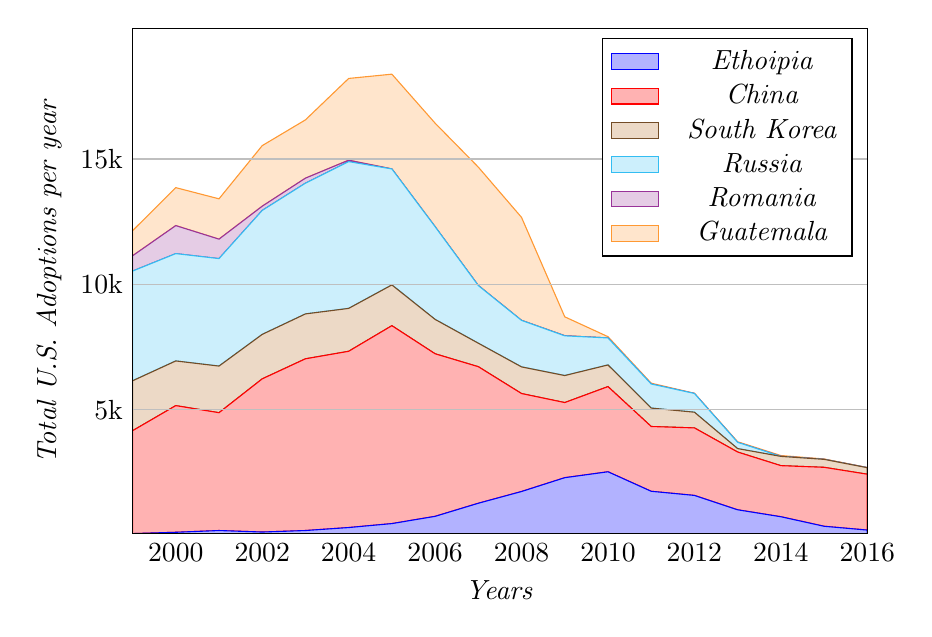
\begin{tikzpicture}
	\begin{axis}[
		stack plots=y,
		area style,
		enlarge x limits=false,
		enlarge y limits=upper,
		width=0.9\textwidth,
		height=8cm,
		xlabel = \textit{Years},
         ylabel = \textit{Total U.S. Adoptions per year},
         ytick = {5000, 10000, 15000},
         ytick style={draw=none},
         xtick style={draw=none},
         yticklabel = {\pgfmathparse{\tick/1000}\pgfmathprintnumber{\pgfmathresult}k},
         x tick label style={/pgf/number format/.cd,%
          scaled x ticks = false,
          set thousands separator={},
          fixed},
         y tick label style={/pgf/number format/.cd,%
          scaled y ticks = false,
          set thousands separator={},
          fixed},
         ymajorgrids=true,
         legend style={column sep=8pt}]
	\addplot coordinates
		{(1999,42) (2000,95) (2001	,165) (2002,105) (2003,165)( 2004,284) (2005,442) (2006,731) (2007	,1254)(2008,1723) (2009,2275) (2010,2511) (2011,1732) (2012,1567) (2013,993) (2014,716) (2015,335) (2016,183)} 
		\closedcycle;
	\addplot coordinates
		{(1999, 4108) (2000, 5058) (2001, 4705) (2002, 6116) (2003, 6857) (2004, 7038) (2005, 7903) (2006, 6492) (2007, 5453) (2008, 3912)  (2009, 3000)  (2010, 3401) (2011, 2587) (2012, 2696) (2013, 2306) (2014, 2040) (2015, 2354) (2016, 2231)}
		\closedcycle;
		\label{figdata:china}
		\addplot coordinates
		{(1999, 1994) (2000, 1784) (2001, 1862) (2002	, 1776) (2003, 1793) (2004, 1713) (2005, 1628) (2006, 1373) (2007, 938) (2008, 1064) (2009, 1079) (2010, 865) (2011, 736) (2012, 627) (2013, 138) (2014	, 370) (2015, 318) (2016, 260)}
		\closedcycle;
		\addplot [draw={cyan!80!white},fill={cyan!20!white}] coordinates
		{(1999, 4381) (2000, 4286) (2001, 4292) (2002, 4950) (2003, 5221) (2004, 5862) (2005, 4631) (2006, 3702) (2007, 2303) (2008, 1857) (2009, 1586) (2010, 1079) (2011, 962) (2012, 749) (2013, 250) (2014, 2) (2015, 0) (2016, 0)}
		\closedcycle;
		\addplot [draw={violet!80!white},fill={violet!20!white}] coordinates
		{(1999, 611) (2000, 1119) (2001, 777) (2002, 169) (2003, 200) (2004, 57) (2005, 2) (2006, 0) (2007, 3) (2008, 2) (2009, 5) (2010, 0) (2011, 0) (2012, 0) (2013, 0) (2014, 3) (2015, 3) (2016, 5)}
		\closedcycle;
		\addplot [draw={orange!80!white},fill={orange!20!white}] coordinates
		{(1999, 1002) (2000, 1516) (2001, 1610) (2002, 2419) (2003, 2328) (2004, 3264) (2005, 3783) (2006, 4135) (2007, 4726) (2008, 4112) (2009, 754) (2010, 50) (2011, 32) (2012, 7) (2013, 23) (2014, 29) (2015, 13) (2016, 2)}
		\closedcycle;
		\label{figdata:guatemala}
		\legend{\textit{Ethoipia},\textit{China},\textit{South Korea},\textit{Russia},\textit{Romania},\textit{Guatemala}}
	\end{axis}
\end{tikzpicture}
\caption{Adoptions to US by top countries from 1999 to 2016.}
\source{U.S. State Department}
\label{fig:usadoptionsdropping}
\end{figure}

As policies change, it's often stated that it's in \textit{``the best interest of the child"}, a point usually supported by strong media-driven high-profile infantile abuse or neglect cases. These incidents are rare, though: only a 0.03\% rate. The rates of child abuse in the countries of origin, on the other hand, are often higher. For example, Russia's rate is about 25 times higher. Such statistics call into question whether the child's best interest is really why countries have been cancelling international adoption. Authors have found that political pressures and international embarrassment can spur countries to halt adoptions. After the \textit{moratorium} on foreign adoptions in Guatemala, a former member of the country's National Adoption Council expressed pride. \textit{``Our image as being the number one exporter of children has changed"}, he said. \textit{``Guatemala has dignity, again"}, he added.

Moreover, developing countries often struggle to meet \textit{The Hague Convention policy}'s high standards, which include creating a central adoption authority, accrediting local agencies and tightening approval procedures, making such a rigorous international regulation more expensive. Fees have been applied to agencies, adoptive parents, orphanages, and countries. This 1993 global agreement, signed by 103 countries in 2016, which meant to make adoption safer and more straightforward, has contributed to their decline.

Foreign adoptions can't solve global poverty, but ending them merely punishes thousands of vulnerable kids and their potential parents worldwide. And that's in nobody's best interest.

\subsection{International adoption in Italy}\label{sub:intadoptioninitaly}
According to \cite{notonlyinfectious}, \cite{nonsoloinfezioni} and \cite{cai2014}, in 2015 Italy was the European country with the highest rate of adoptions and the second one worldwide, following the United States. This dominant role was confirmed in the next two-year period: 2.716 children were adopted from foreign countries in 2016-2017 (see \cite{cai2016}), keeping Italy second worldwide for international custody transfers (see \cite{adoptdropping_article} and \cite{adoptdropping_book}).
As of \cite{unreport}, in 1999 Italy was the fourth country worldwide for international adoptions with 2.177 international adoptions, amounting to 68\% of national total. Most of the Italian adoptees are from the Russian Federation (as shown in Table \ref{tab:intadoptcountriesdestination}) and Italy is Bulgaria's favorite country of destination (in Table \ref{tab:intadoptcountriesorigin}).

%International adoption countries of destination
\begin{table}[H]
   \centering
   \begin{tabular}{l c r r c r r}
      & & \multicolumn{2}{c}{Year 2016} & & \multicolumn{2}{c}{Year 2017}\\
      \cline{3-4} \cline{6-7}
      Region & & Value & Percentage & & Value & Percentage\\
      \hline
      Lombardia & & 258 & 16,7 & & 179 & 15,3\\
      Veneto & & 151 & 9,8 & & 125 & 10,7\\
      Lazio & & 145 & 9,4 & & 112 & 9,6\\
      Toscana & & 144 & 9,3 & & 124 & 10,6\\
      Campania & & 132 & 8,5 & & 99 & 8,5\\
      Puglia & & 123 & 7,9 & & 85 & 7,3\\
      Emilia-Romagna & & 119 & 7,7 & & 86 & 7,4\\
      Piemonte & & 93 & 6,0 & & 69 & 5,9\\
      Sicilia & & 68 & 4,4 & & 44 & 3,8\\
      Calabria & & 55 & 3,6 & & 37 & 3,2\\
      Liguria & & 52 & 3,4 & & 39 & 3,3\\
      \textcolor{BrickRed}{\textbf{Friuli-Venezia Giulia}} & & \textcolor{BrickRed}{\textbf{43}} & \textcolor{BrickRed}{\textbf{2,8}} & & \textcolor{BrickRed}{\textbf{34}} & \textcolor{BrickRed}{\textbf{2,9}}\\
      Marche & & 42 & 2,7 & & 39 & 3,3\\
      Umbria & & 29 & 1,9 & & 20 & 1,7\\
      Trentino-Alto Adige & & 26 & 1,7 & & 18 & 1,5\\
      Sardegna & & 26 & 1,7 & & 17 &1,5 \\
      Abruzzo & & 20 & 1,3 & & 28 & 2,4\\
      Basilicata & & 13 & 0,8 & & 85 & 7,3\\
      Molise & & 9 & 0,6 & & 1 & 0,1\\
      Valle d'Aosta & & 0 & 0,0 & & 0 & 0,0\\
      \hline
      Total & & 1.548 & 100 & & 1.168 & 100\\
   \end{tabular}
   \caption{Intercountry adoptions by Italian regions, years 2016 and 2017.}
    \source{Italian Presidency of Council of Ministers, Commission for International Adoptions. See \cite{cai2016}.}
    \label{tab:italianregions}
\end{table}

Table \ref{tab:italianregions} shows that Lombardia, Veneto, and Lazio were the leading Italian regions for international adoption in 2016-2017, followed by Toscana and Campania. \textit{De facto}, the northern and central portions of the country are the most mobile adoption-wise.  Overall and regional numbers are dropping, in the same manner as it is happening all over the globe, as explained in Section \ref{sub:levelsintercountry}, but a few exceptions stand out. Abruzzo and Basilicata increased their annual adoptions, from 20 to 28, the first, and from 13 to 85, the latter. Even more exceptional is Valle d'Aosta, that scored a flat \textit{zero} in both years. It must be said, though, that it's the least populated region of the country, with only 125.000 people living in the whole region.

Most of these children, between 40 and 50\%, span between 5 and 9 years of age at their arrival in Italy, and less than 15\% are extremely young (younger than one year-olds) or older than 10 years old. 

In 2016 and 2017, the most fertile countries of origin are the same in both years, even though they swap internal ratings: Russian Federation, Colombia, India, Hungary, Poland, Vietnam, Brazil, and China (as stated in \cite{cai2016}). The children originating from these countries amount to almost 73\% of the total international adoptions.

\section{Role of the pediatrician}\label{sec:roleofpediatrician}
Internationally adopted children come from countries with many infectious endemic diseases, including hepatitis B, tuberculosis and many different intestinal parasites (as explained in \cite{caringfor}). These children have lived in crowded conditions, sometimes with poor standards of hygiene and inadequate nutrition. Most of the times they are malnourished, often suffer from emotional and physical neglect, environmental deprivation, and are, therefore, vulnerable to infectious diseases. Although children must obtain medical clearance as part of the process of applying for a visa to travel around the globe, the evaluation is usually cursory, thus unreliable. The physician appointed to establish this sketchy health status certificate is directed to evaluate the child for \textit{``serious contagious diseases or disabilities"}. However, no blood testing is required or other screening is mandated unless risk factors are identified.

According to \cite{medicalscreening}, more than 50\% of internationally adopted children, regardless of sex, age, and country of origin, will have a previously undiagnosed medical condition, which is identified on initial evaluation. Therefore, adoption-medicine specialized pediatricians should advise prospective parents on appropriate testing of the child after arrival in the country of destination. Early screening is crucial in order to identify eventual pathological conditions and prevent what could be irreversible damage. Many studies (\textit{a.e.} see \cite{notonlyinfectious} and \cite{obringer}) have assessed prevalence of infectious diseases, ranging between 35 and 42\% for all infections, almost 40\% for parasitic infestations (see \cite{GNLBIexp} and \cite{sollai}), and between 5 and 19\% for tuberculosis (see \cite{sollai} and \cite{ampofo}).\\
As can be found in \cite{initialeval}, \cite{redbook}, \cite{GNLBIexp}, and the more recent \cite{comphealtheval}, the American Academy of Pediatrics recommends careful health screening of all newly arrived international adoptees.

Reference \cite{nelson} states that the results of specific diagnostic studies and laboratory tests performed in the country of origin should not be relied on and should be repeated once the child arrives in the country of destination. Paradoxically, review of the child’s medical records may raise more questions than provide answers, because of poor translation and use of medical terminology and medications that are unfamiliar to physicians trained in the country of destination. Each medical diagnosis should be considered carefully before being rejected or accepted.

\textit{Therefore, what screening tests should be ordered by physicians caring for newly arrived international adoptees?} In addition to hepatitis A, B and C, HIV, congenital syphilis, other STIs, intestinal parasites, and tuberculosis by Mantoux testing, experts also recommend testing for anemia, thyroid and renal disease, vision and hearing defects, and newborn metabolic disorders when appropriate, along with careful monitoring of growth and development (according to \cite{caringfor}, \cite{medicalscreening}, \cite{notonlyinfectious}, and \cite{nonsoloinfezioni}). In this matter, particular attention should be paid to Feto Alcohol Spectrum Disorders (FASD), as \cite{notonlyinfectious} and \cite{nonsoloinfezioni} suggest; according to these studies, more than 17\% of all internationally adopted children evidenced special needs, in which FASD is the most common condition observed. Chansoff \textit{et al.} in \cite{misdiagnosis}, in a sample of 547 foster and adopted children reported that 86.5\% children with FASD had never been previously diagnosed. Particular attention should be paid to children originating from Russia.\\
Moreover, \cite{caringfor}, \cite{medicalscreening}, \cite{initialeval}, \cite{immunizationstatus}, \cite{comphealtheval}, and \cite{immunizationstillinsufficient} are only some of the examples of a medical literature full to the brim, which compels physicians to test for adequate immunization status for vaccine-preventable disease. Pre-adoptive immunization records may not be assumed as truthful or correct, according to \cite{immunizationstatus}. As discussed in \cite{comphealtheval}, this may happen because the \textit{cold chain} gets interrupted, vaccines are used beyond expiration dates, they are poorly stored or they are incorrectly given, too early or too far apart. Therefore, guidelines suggest that all internationally adopted children, with or without any official immunization records, should always be tested for their immunization status as soon as they come to the adopting country, in order to perform vaccinations whether serum antibody titers are inadequate. At this regard, Italian laws (see \cite{circolareministeriale} and \cite{centroprevenzione}) suggest re-vaccinating subjects who have unknown, incomplete or undocumented vaccination status, without even checking for residual immunization.\\
As \cite{preventing} points out, families of internationally adopted children face risks associated with travel if they pick up their children overseas. Unlike other travelers, though, they also face risks because of close contact with a child with uncertain infection and vaccination status. Some of these transmissible infections may be inapparent or may not be manifest in adopted children until many years after the adoption, posing risks to the well-being of these children's new families and communities.

Although concern about HIV infection causes considerable anxiety amongst the general population, very few internationally adoptees  were found positive to HIV testing (see \cite{caringfor}). Either HIV-infected children do not survive long enough to complete an international adoption procedure or local screening identifies infected children and removes them from consideration for adoption.

Internationally adopted children have often experience pre- and perinatal complications, such as exposure to drugs and alcohol during gestation, the absence of perinatal care, low birth weight, and prematurity (see \cite{preventing}). Although this is widely known and well documented, several systematic reviews and eminent periodicals focused on infectious disease risk among internationally adopted children. Data regarding prevalence and spectrum of non-infectious conditions, including special needs, FASD and labio-palatal schisis, are poor (see \cite{notonlyinfectious} and \cite{nonsoloinfezioni}). At the time of adoption, many children exhibit delays in at least one area of development, but most exhibit significant gains within the first 12 months after adoption. Those adopted before 6 months of age usually demonstrate typical development, whereas those adopted at older ages have more variable outcomes (see \cite{nelson}). Careful monitoring of development within the first year of adoption can identify a ``developmental trend" over time that may be more predictive of long-term functioning than assessment at any specific point in time. 

One medical peculiarity is that even in the most recent literature reviews concerning international adoptees' health evaluation, vitamin D serum levels are usually left out. This is contradictory with many other papers (see \cite{vitDadopt1}, \cite{vitDadopt2}, \cite{vitDadopt3}, and \cite{vitDadopt4}) that strongly advise towards the relevance of this test for the well being of the child. Internationally adopted children often suffer from vitamin D deficiency or insufficiency, because of the profound change in latitude they experience during the adoption phase, or because of malnutrition combined with lack of solar exposure during pre-adoptive care, usually in orphanages.\\
There is no reasonable doubt that vitamin D deficit is one of the most relevant medical issues among internationally adopted children and it is mandatory for the pediatrician to test and appropriately treat this disorder.

Table \ref{tab:AAPrecscreening} summarizes the recommendations of the American American Academy of Pediatrics (source: \textit{Nelson - Textbook of Pediatrics}, \nth{20} Edition. See \cite{nelson}), as follows:

%Setting mylength
\newlength\mylength
\setlength\mylength{\dimexpr\textwidth-5\arrayrulewidth-8\tabcolsep}

%International adoption countries of destination
\vspace{0.5cm}
\begin{footnotesize}
    \centering
	\begin{longtable}{p{0.5\mylength} p{0.5\mylength}}
	   	 \hline
	      \multicolumn{2}{c}{\small{\textbf{Screening tests}}}\\
	      \hline
	      \multicolumn{2}{l}{Complete blood cell count}\\
	      \multicolumn{2}{l}{Haemoglobin identification}\\
	      \multicolumn{2}{l}{Blood lead level}\\
	      \multicolumn{2}{l}{Urinalysis}\\
	      \multicolumn{2}{l}{Newborn screening\footnotemark[2]}\\
	      \multicolumn{2}{l}{Vision and hearing screening}\\
	      \multicolumn{2}{l}{Developmental testing}\\\\
	      \multicolumn{2}{l}{\textit{Other screening tests to consider based on clinical findings and age of the child}}\\
	      \multicolumn{2}{l}{Detection of \textit{Helicobacter pylori} antibody \textit{or} $^{13}$C-urea breath test}\\
	      \multicolumn{2}{l}{Stool cultures for bacterial pathogens}\\
	      \multicolumn{2}{l}{\textit{Glucose-6-phosphate dehydrogenase} deficiency screening}\\
	      \multicolumn{2}{l}{Sickle cell}\\
	      \multicolumn{2}{l}{Urine pregnancy test}\\ \noalign{\penalty-5000}
	      \hline
	      \multicolumn{2}{c}{\small{\textbf{Screening tests for infectious diseases}}}\\*
	      \hline
	      \textit{Recommended tests} & \textit{Optional tests}\\
	      Hepatitis B virus serologic testing: \textit{HBsAg and anti-HBs Ab}\footnotemark[3] & Neisseria gonorrhoeae and Chlamydia trachomatis testing\\
	      Hepatitis C virus serologic testing\footnotemark[3] & Chagas disease serology\\
	      Hepatitis A virus serologic testing & Malaria thick and thin smears\\
	      Varicella virus serologic testing & Urine for O\&P for schistosomiasis\footnotemark[4]\\
	      Syphilis serologic testing: Treponemal and Non-treponemal tests & \\
	      Human immunodeficiency viruses 1 and 2 testing\footnotemark[3]$^{,}$\footnotemark[5] & \\
	      Complete blood cell count with red blood cell indices and differential & \\
	      Stool examination for ova and parasites (2 or 3 specimens) & \\
	      Stool examination for \textit{Giardia lamblia} and \textit{Cryptosporidium} antigen (1 specimen) & \\
	      Tuberculin skin test or interferon-$\gamma$ release assay\footnotemark[3]$^{,}$\footnotemark[6] & \\
	   \caption{American Academy of Pediatrics' recommended screening tests for international adoptees upon U.S. Arrival}
	    \label{tab:AAPrecscreening}
	\end{longtable}
\end{footnotesize}

\footnotetext[2]{Only for children younger than 12 months of age.}
\footnotetext[3]{To be repeated 3-6 months after arrival.}
\footnotetext[4]{Only if hematuria is present.}
\footnotetext[5]{ELISA if the child is older than 18 months; PCR if he or she is younger than 18 months.}
\footnotetext[6]{Followed by a chest X-ray if the text results in hive or induration are bigger than 5 \si{\milli\metre}}

Lastly, the sanitary surveillance on internationally adopted children, both clinical and test-based, is based in Italy in 20 centers, one per region. In Friuli-Venezia Giulia, this center is placed in \textit{San Vito al Tagliamento}, where the data for this paper has been collected. For a more in-depth overview of the work they do on a day-to-day basis, see the Introduction to Chapter \ref{chap:materialsandmethods} on page \pageref{chap:materialsandmethods}.

\subsection{Watch out for the \textit{fragile creature}}
On the other hand, pediatricians must be warned about the psychosocial risks derived from considering an adoptee as such a \textit{fragile creature}. As illustrated in \cite{initialeval}, prior to adoption, or at the time of entry into the family unit, the pediatrician should begin a careful medical assessment of the child and should counsel the family appropriately regarding adoption issues. Pediatricians should be alert to the following potential problems:

\begin{enumerate}
    \item Some parents expect the guarantee of a \textit{``perfect child"}. They may push for unnecessary tests and expect unrealistic predictions from the pediatrician. Just as a birth family cannot be certain that its natural child will be healthy, the adoptive family cannot be guaranteed that a child will not have future health problems.
    \item By focusing on an extensive medical evaluation of a child, the pediatrician must be careful not to create a \textit{``vulnerable child"} through an exaggerated assessment of historical risk. Most adopted children are healthy, or at least can become so, even if they come from high-risk backgrounds. Certainly, the risks must be defined and then carefully explained to the family, so that problems can be anticipated and dealt with expediently. This is the same anticipatory guidance the pediatrician uses for all patients.
    \item It is not the pediatrician's role to judge the advisability of a proposed adoption, but it is appropriate and necessary that the prospective parents and any involved agency be apprised clearly and honestly of any special health needs detected now or anticipated in the future.
\end{enumerate}

Thus, the pediatrician should resist unreasonable demands while still being empathic with the adoptive parents' anxieties and concerns.

%\section{Illnesses and dysfunctions under exam}\label{sec:illnessesanddysfunctions}
%Lorem ipsum dolor sit amet, consectetur adipiscing elit. Pellentesque nibh metus, suscipit a scelerisque sit amet, rhoncus et lectus. Mauris eget erat rutrum, euismod massa id, maximus mauris. Nulla maximus, ex sit amet lacinia consequat, enim ante mollis dui, sit amet tincidunt massa felis id magna. Aenean gravida ante nec volutpat rutrum. Cras eget ullamcorper leo. Curabitur eu volutpat tellus. Integer nec ornare sapien. Fusce ipsum justo, interdum quis libero a, mattis tristique velit. Phasellus rhoncus lorem non ultrices luctus.

%DI CIASCUNA INSERISCI EPIDEMIOLOGIA E FISIOPATO

%\subsection{Infectious diseases}\label{sub:infectiousdiseases}
%Lorem ipsum dolor sit amet, consectetur adipiscing elit. Pellentesque nibh metus, suscipit a scelerisque sit amet, rhoncus et lectus. Mauris eget erat rutrum, euismod massa id, maximus mauris. Nulla maximus, ex sit amet lacinia consequat, enim ante mollis dui, sit amet tincidunt massa felis id magna. Aenean gravida ante nec volutpat rutrum. Cras eget ullamcorper leo. Curabitur eu volutpat tellus. Integer nec ornare sapien. Fusce ipsum justo, interdum quis libero a, mattis tristique velit. Phasellus rhoncus lorem non ultrices luctus.

%\subsubsection{Tuberculosis}\label{sub:tbc} it can occur.
%See 7.3 {caringfor} p. 1540

%\subsection{Blood count disorders and deficiency states}\label{sub:bloodcountdisorders}
%Lorem ipsum dolor sit amet, consectetur adipiscing elit. Pellentesque nibh metus, suscipit a scelerisque sit amet, rhoncus et lectus. Mauris eget erat rutrum, euismod massa id, maximus mauris. Nulla maximus, ex sit amet lacinia consequat, enim ante mollis dui, sit amet tincidunt massa felis id magna. Aenean gravida ante nec volutpat rutrum. Cras eget ullamcorper leo. Curabitur eu volutpat tellus. Integer nec ornare sapien. Fusce ipsum justo, interdum quis libero a, mattis tristique velit. Phasellus rhoncus lorem non ultrices luctus.

%INSERISCI LA NORMALITÀ

%\subsubsection{Iron-deficient anemia}\label{sub:iron-deficiency} it can occur.
%Segna qui le cause più frequenti: sideropenia, talassemia, perdita da parassiti.

%\subsubsection{Vitamin D deficiency}\label{sub:vitaminddeficiency} it can occur too.

%\subsection{Height-weight disorders}\label{sub:heightweightdisorders}
%Lorem ipsum dolor sit amet, consectetur adipiscing elit. Pellentesque nibh metus, suscipit a scelerisque sit amet, rhoncus et lectus. Mauris eget erat rutrum, euismod massa id, maximus mauris. Nulla maximus, ex sit amet lacinia consequat, enim ante mollis dui, sit amet tincidunt massa felis id magna. Aenean gravida ante nec volutpat rutrum. Cras eget ullamcorper leo. Curabitur eu volutpat tellus. Integer nec ornare sapien. Fusce ipsum justo, interdum quis libero a, mattis tristique velit. Phasellus rhoncus lorem non ultrices luctus.

%INSERISCI LA NORMALITÀ